\documentclass[../../thesis.tex]{subfiles}

\begin{document}
\TODO{Should i elaborate on anything? Feels a bit brief, but i am kinda stuck}

Our work in this thesis, as mentioned earlier, builds upon the paper "Vector Quantized Time Series Generation with a Bidirectional Prior Model" \cite{TimeVQVAE}. We simplify the model architecture by omitting the high-low frequency split, reducing the model to what they refer to as naive TimeVQVAE in their paper. We expand upon naive TimeVQVAE by integrating a self-supervised learning (SSL) extension. \newline

A schematic figure of our proposed tokenization model is given in Figure \ref{fig:NCVQVAE}. To encode semantic information into the discrete latent representation and improve class separation, we introduce a non-contrastive self-supervised loss. The intuition is that the SSL loss pushes the representations of original and augmented views closer together, which should structure the discrete latent space in such a way that data with similar characteristics inhabit distinct regions. Additionally, we add a regularizing term by reconstructing augmented views. We hypothesize that this approach enables the model to generalize better to unseen data by allowing the decoder to "see" the augmented views, as well as preventing the encoder from ignoring the augmentations.

\section{Proposed model: NC-VQVAE}

Our model, termed NC-VQVAE, is a generative time series model that learns expressive discrete latent representations by combining VQVAE with non-contrastive SSL algorithms. NC-VQVAE uses the two-stage modeling approach and can be considered an extension of their naive TimeVQVAE. Our model primarily extends the tokenization stage, incorporating Barlow Twins and VIbCReg as our non-contrastive SSL methods, while the framework remains flexible. For the second stage, we model the prior using a bidirectional transformer similar to MaskGIT.

\subsection{Stage 1: Tokenization}
\TODO{Pseudocode}

The architecture of the tokenization model, shown in Figure \ref{fig:NCVQVAE}, consists of two branches: the original and augmented branch. The model takes a time series $x$ as input and creates an augmented view $x'$. The original branch follows the naive TimeVQVAE architecture from \cite{TimeVQVAE}, while the augmented branch is an autoencoder, constructed by omitting the quantization layer. The views are passed through their respective branches, and we compute the SSL loss derived from the original discrete latent representation $z_q$ and the augmented continuous latent $z'$, before the decoder reconstructs each latent representation. \newline 

The SSL loss is calculated by concatenating the global average and max pool of both representations individually and passing the resulting vectors through the projector.\newline

\begin{figure}[h]
    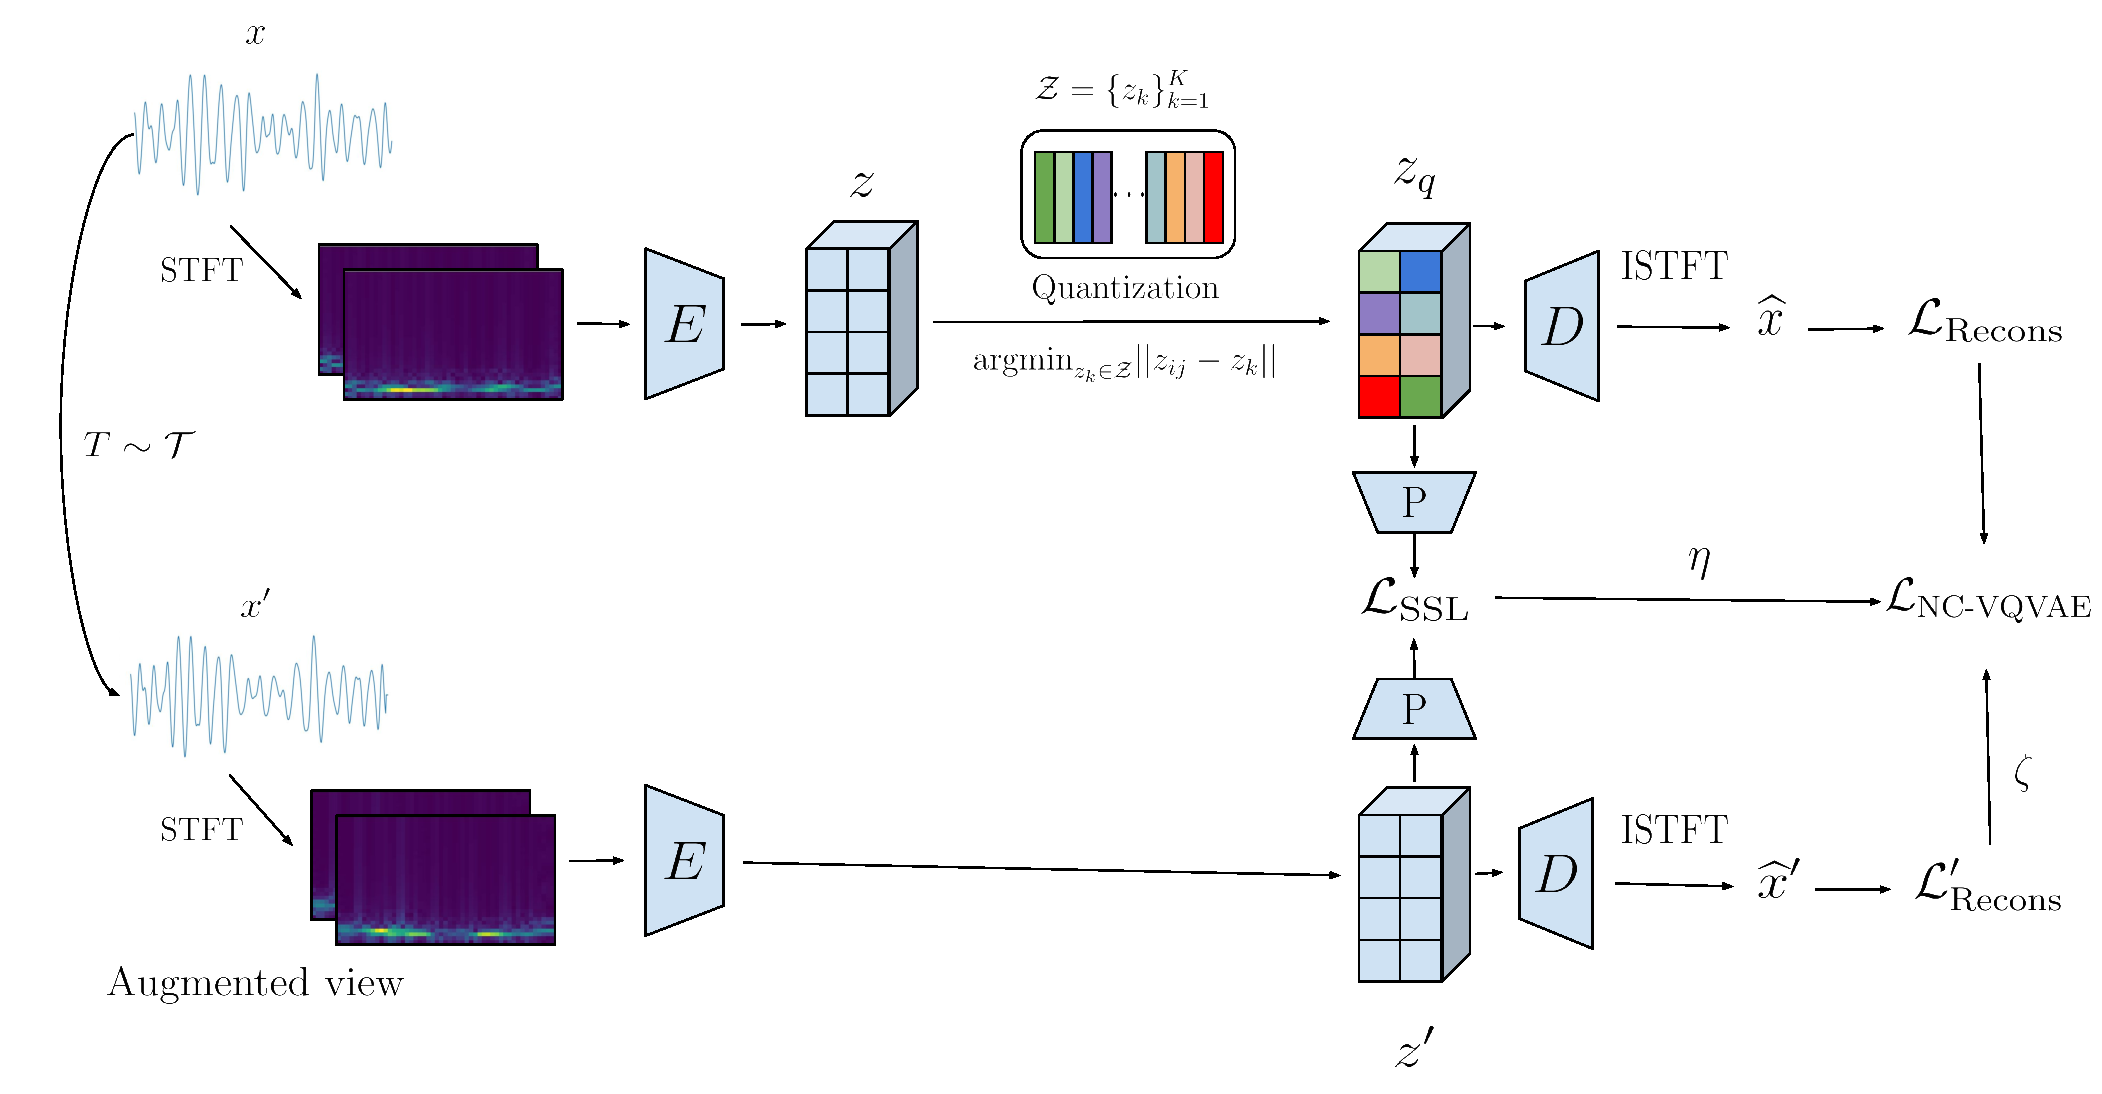
\includegraphics[scale=0.35]{Siam-VQVAE.pdf}
    \centering  
    \caption{Overview of proposed model: NC-VQVAE.}
    \label{fig:NCVQVAE}
\end{figure}

\subsubsection{Loss}
Our training objective mirrors the training objective from TimeVQVAE in equation \ref{eq:TimeVQVAE_loss}, without the frequency split. Our contribution is the addition of an SLL loss together with a reconstruction loss on the augmented branch.\newline

To refresh the reader's memory, the VQ loss consists of a reconstruction loss and a codebook loss, which is the Euclidean distance between continuous and discrete latent representations, along with a commitment loss to prevent the codewords from diverging. In our setup, the codebook loss reduces to
\begin{equation}
    \label{eq:NCVQVAE_codebook}
    \begin{aligned}
        \loss_\text{codebook} &= ||\sg[z] - z_q ||_2^2 \\
                              &+ \beta||z - \sg[z_q]||_2^2,
    \end{aligned}
\end{equation}
and the reconstruction loss to
\begin{equation}
    \label{eq:NCVQVAE_recons}
        \loss_\text{recons} = ||x - \widehat{x} ||_2^2 + ||u - \widehat{u}||_2^2.
\end{equation}

Our VQ loss is then given by
\begin{equation}
    \label{eq:NCVQVAE_loss}
    \loss_\text{VQ} = \loss_\text{codebook} + \loss_\text{recons}.
\end{equation}

The SSL loss varies depending on the SSL method used. It is calculated on derived values from $z_q$ and $z'$. We consider Barlow Twins \ref{eq:BTLoss} and VIbCReg \ref{eq:VIbCRegLoss}, both of which utilize a projector. We apply a global average and max pool operation on both tensors and pass them through the projector before calculating the SSL loss.\newline


The augmented reconstruction loss is simply given as 
\begin{equation}
    \label{eq:NCVQVAE_augrecons}
        \loss_\text{recons}' = ||x' - \widehat{x}' ||_2^2 + ||u' - \widehat{u}'||_2^2.
\end{equation}

This loss ensures that the encoder and decoder reconstruct the augmented view, which, in conjunction with the SSL loss, influences the codebook to encode information regarding the augmentations. Additionally, it helps prevent the encoder from ignoring reconstruction in favor of the SSL loss. Initial experiments showed that omitting the augmentation reconstruction led to severe overfitting.\newline

The total loss is given by 
\begin{equation}
    \loss_{NC-VQVAE} = \loss_{VQ} + \eta\loss_{\text{SSL}} + \zeta \loss_\text{recons}',
\end{equation}
where $\eta$ and $\zeta$ are hyperparameters influencing the importance of each term in the total training objective. An illustration of the effect of the different loss terms on the latent space during training is presented in Figure \ref{fig:NCVQVAE_losses}. 

\begin{figure}
    \centering
    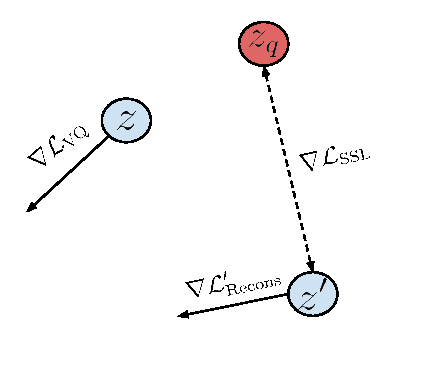
\includegraphics[scale = 0.7]{NCVQVAE_losses.pdf}
    \caption{Illustration of the effect of different loss terms during training.}
    \label{fig:NCVQVAE_losses}
\end{figure}

\subsection{Stage 2: Prior learning}

In our model, the input embedding for the bidirectional transformer is initialized with the codebook, which has additional structure from the SSL loss. Instead of introducing an additional masking vector in the embedding matrix, we use the codebook directly and create a separate learnable masking vector to mask the embedded sequences. In order to separate this masking vector, we do the embedding stage before masking, effectively factoring the embedding out of the transformer. This approach ensures that the learning of the masked token embedding is independent of the other embeddings, further leveraging the learned codewords from stage 1 without unnecessary influence. Except for this adjustment, and the possibility of class conditional sampling from TimeVQVAE, our method is equivalent to MaskGITs.
\newline

The process for generating samples at inference time follows the same iterative steps as MaskGIT, ensuring robust and high-quality sample generation.



\end{document}